% ID: SEL-D0017-BA-E01
% ESTADO: validada. S018. Revisión matemática, didáctica y visual.
\textbf{Modelo y recinto factible.}\par\nopagebreak[4]
Sean $x$ las tartas de chocolate e $y$ las de merengue y chocolate. Los límites de bizcocho, crema y merengue, respectivamente, dan
\[
x+2y\le100,\qquad 2x+y\le80,\qquad y\le46,\qquad x,y\ge0.
\]
Se maximiza $F(x,y)=10x+12y$, en euros. Las cantidades de tartas son enteras. Podemos estudiar primero el recinto continuo y comprobar que su máximo se alcanza con cantidades enteras.

Los cortes factibles de las fronteras son, en orden,
\[
(0,0),\quad(40,0),\quad(20,40),\quad(8,46),\quad(0,46).
\]
Los dos recursos compartidos se agotan simultáneamente en $(20,40)$. La frontera del merengue corta a la del bizcocho en $(8,46)$.
\begin{center}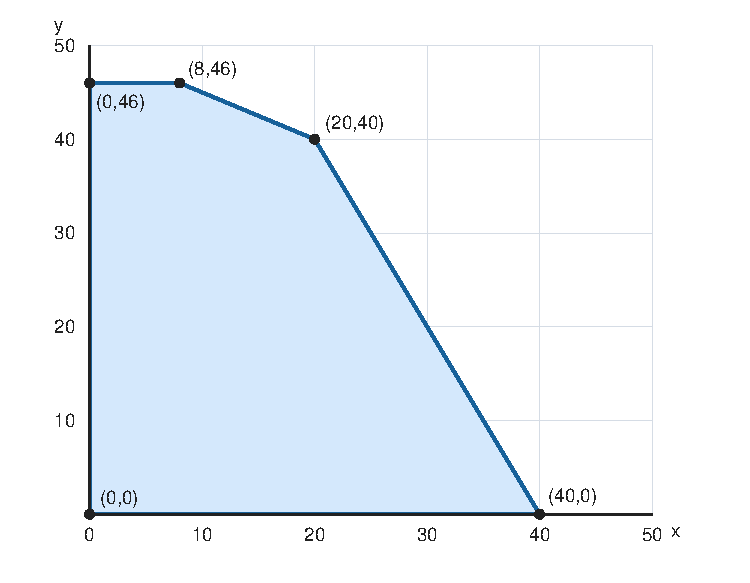
\includegraphics[width=0.53\linewidth]{recursos/figuras/s018-region.pdf}\end{center}
Los beneficios en los vértices son $0$, $400$, $680$, $632$ y $552$ euros. Además,
\[
F=\frac{14}{3}(x+2y)+\frac83(2x+y)\le\frac{1400+640}{3}=680.
\]
Ambas restricciones deben ser igualdades para alcanzar esta cota. El punto $(20,40)$ cumple todos los límites y proporciona el máximo único:
\[
\boxed{20\text{ tartas de chocolate},\quad40\text{ de merengue y chocolate},\quad680\text{ euros}.}
\]
